% ~~~~~~~~~~~~~~~~~~~~~~~~~~~~~~~~~~~~~~~~
%% INTRODUCTION
% ~~~~~~~~~~~~~~~~~~~~~~~~~~~~~~~~~~~~~~~~
\chapter{Introduction}
The Simulation Experiment Description Markup Language (SED-ML) is an XML-based format for the description of simulation experiments.

The number of computational models of biological systems is growing at an ever increasing pace. 
At the same time, their size and complexity are also increasing. It is now generally accepted that one must be able to exchange the mathematical structure of such models, for instance to build on existing studies by reusing models or for the reproduction of model results. The efforts to standardize the representation of computational models in various areas of biology, such as the Systems Biology Markup Language (SBML) \citep{Hucka:2003}, CellML \citep{cuellar:2003} or NeuroML \citep{Goddard:2001}, resulted in an increase of the exchange and re-use of models. 

However, the description of the structure of models is not sufficient for the reproduction of simulation results. One also needs to describe the procedures the models are subjected to, i.e., the information that must be provided to allow the reproduction of simulation experiments among users and software tools. The increasing use of computational simulation experiments to inform modern biological research creates new challenges to reproduce, annotate, archive, and share such experiments. 

SED-ML describes in a computer-readable exchange format the information to enable the reproduction of simulation experiments. SED-ML is a software-independent format encoded in the Extensible Markup Language (XML) not specific to particular simulation tools and independent of the underlying model implementation. SED-ML describes the minimum information of a simulation experiment as described by the Minimum Information About a Simulation Experiment (MIASE) \citep{Waltemath:2011}.

SED-ML is developed as a community project and defined via a detailed technical specification and a corresponding XML Schema. 

This document describes \currentLV of SED-ML which is the successor of \previousLV and \LoneVone (described in \citep{WAB+11}).

% ~~~~~~~~~~~~~~~~~~~~~~~~~~~~~~~~~~~~~~~~
%% OVERVIEW
% ~~~~~~~~~~~~~~~~~~~~~~~~~~~~~~~~~~~~~~~~
\section{SED-ML overview}
SED-ML specifies for a given simulation experiment

\begin{itemize}
\item what datasets to use (\hyperref[class:dataDescription]{DataDescription}),
\item which models to use (\hyperref[class:model]{Model}),
\item which modifications to apply to models before simulation (\hyperref[class:change]{Change}),
\item which simulation procedures to run on each model (\hyperref[class:simulation]{Simulation} and \hyperref[class:task]{Task}),
\item what analysis results to plot or report and how to post-process the data (\hyperref[class:dataGenerator]{DataGenerator}), and
\item how these results should be presented (\hyperref[class:output]{Output})
\end{itemize}

A \hyperref[class:sed-ml]{SED-ML document} contains the following main objects to describe this information: \hyperref[class:dataDescription]{DataDescription}, \hyperref[class:model]{Model}, \hyperref[class:change]{Change}, \hyperref[class:simulation]{Simulation}, \hyperref[class:task]{Task}, \hyperref[class:dataGenerator]{DataGenerator}, and \hyperref[class:output]{Output}.

\paragraph*{\hyperref[class:dataDescription]{DataDescription}}
The \hyperref[class:dataDescription]{DataDescription} class allows to specify datasets used in a simulation experiment. Such data can be used for instance for parametrization of model simulations or to plot data with simulation results.

\paragraph*{\hyperref[class:model]{Model}}
The \hyperref[class:model]{Model} class allows to reference the models used in a simulation experiment.

The \hyperref[class:change]{Change} class allows to modify models (pre-processing), i.e., changing the value of an observable, computing the change of a value using mathematics, or general changes on any XML element of the model representation that is addressable by \hyperref[sec:xpath]{XPath} expressions, e.g., substituting a piece of XML by an updated one.

\paragraph*{\hyperref[class:simulation]{Simulation}}
The \hyperref[class:simulation]{Simulation} class defines the simulation settings and the steps taken during simulation. These include the particular type of simulation, the algorithm, and the algorithm parameters used for the execution of the simulation.

\paragraph*{\hyperref[class:task]{Task}}
SED-ML uses the \hyperref[class:task]{Task} class to specify which \hyperref[class:simulation]{Simulation} is run with which \hyperref[class:model]{Model}.

\paragraph*{\hyperref[class:dataGenerator]{DataGenerator}}
The \hyperref[class:dataGenerator]{DataGenerator} class allows to encode post-processing of simulation results before output, e.g., one might want to normalize a plot before output, or apply post-processing like mean-value calculation. In the definition of a \hyperref[class:dataGenerator]{DataGenerator}, any addressable variable or parameter of any defined model or datasets from \hyperref[class:dataDescription]{DataDescription} may be referenced, and new entities might be specified using \hyperref[sec:mathML]{MathML}.

\paragraph*{\hyperref[class:output]{Output}}
The \hyperref[class:output]{Output} defines the output of the simulation, which can be either a two dimensional plot (\hyperref[class:plot2D]{Plot2D}), a three dimensional plot (\hyperref[class:plot3D]{Plot3D}), or data table (\hyperref[class:report]{Report}). The \hyperref[class:output]{Output} is based on the post-processed simulation results in the \hyperref[class:dataGenerator]{DataGenerators}.

This section provided a low level overview over the content of a simulation experiment in SED-ML. For the detailed technical specification see Chapter~\ref{chp:specification}. 

% ~~~~~~~~~~~~~~~~~~~~~~~~~~~~~~~~~~~~~~~~
%% EXAMPLE SIMULATION
% ~~~~~~~~~~~~~~~~~~~~~~~~~~~~~~~~~~~~~~~~
\section{Example simulation experiment}
\label{motivation:example}
In this section an example simulation experiment in SED-ML is presented for the repressilator model \citep{Elowitz:2000}. The corresponding SED-ML is listed in Appendix~\ref{example:repressilator}, the \hyperref[sec:archive]{Combine Archive} for this simulation experiment is available as \texttt{L1V3\char`_repressilator.omex} from \url{http://sed-ml.org/}.

The repressilator is a synthetic oscillating network of transcription regulators in Escherichia coli. The network is composed of the three repressor genes Lactose Operon Repressor (lacI), Tetracycline Repressor (tetR) and Repressor CI (cI), which code for proteins binding to the promoter of the other, blocking their transcription. The three inhibitions together in tandem, form a cyclic negative-feedback loop. To describe the interactions of the molecular species involved in the network, the authors built a simple mathematical model of coupled first-order differential equations. All six molecular species included in the network (three mRNAs, three repressor proteins) participate in creation (transcription/translation) and degradation processes. The model was used to determine the influence of the various parameters on the dynamic behavior of the system. In particular, parameter values were sought which induce stable oscillations in the concentrations of the system components.

%% ~~ TIME-COURSE ~~
\subsection{Time-course simulation}
\label{sec:timecourse}
The first simulation experiment with the model reproduces the oscillation behavior of the model shown in Figure~1c of the reference publication \citep{Elowitz:2000}. This simulation experiment can be described as:

\begin{enumerate}
 	\item{Import the repressilator model identified by the Unified Resource Identifier (URI) \citep{Berners-Lee:2005}\\ 	\url{urn:miriam:biomodels.db:BIOMD0000000012}.}
 	\item {Select a deterministic simulation method for the numerical integration.}
 	\item{Run a uniform time course simulation for 1000~min with an output interval of 1~min.}
 	\item{Plot the amount of \code{lacI}, \code{tetR} and \code{cI} against time in a 2D Plot.}
 \end{enumerate}

Following those steps and performing the simulation experiment in a simulation tool supporting SED-ML results in the output shown in \fig{rep_tc1} and \fig{rep_tc2}.

\begin{figure}[ht]
    \centering
    \begin{minipage}{0.47\textwidth}
        \centering
        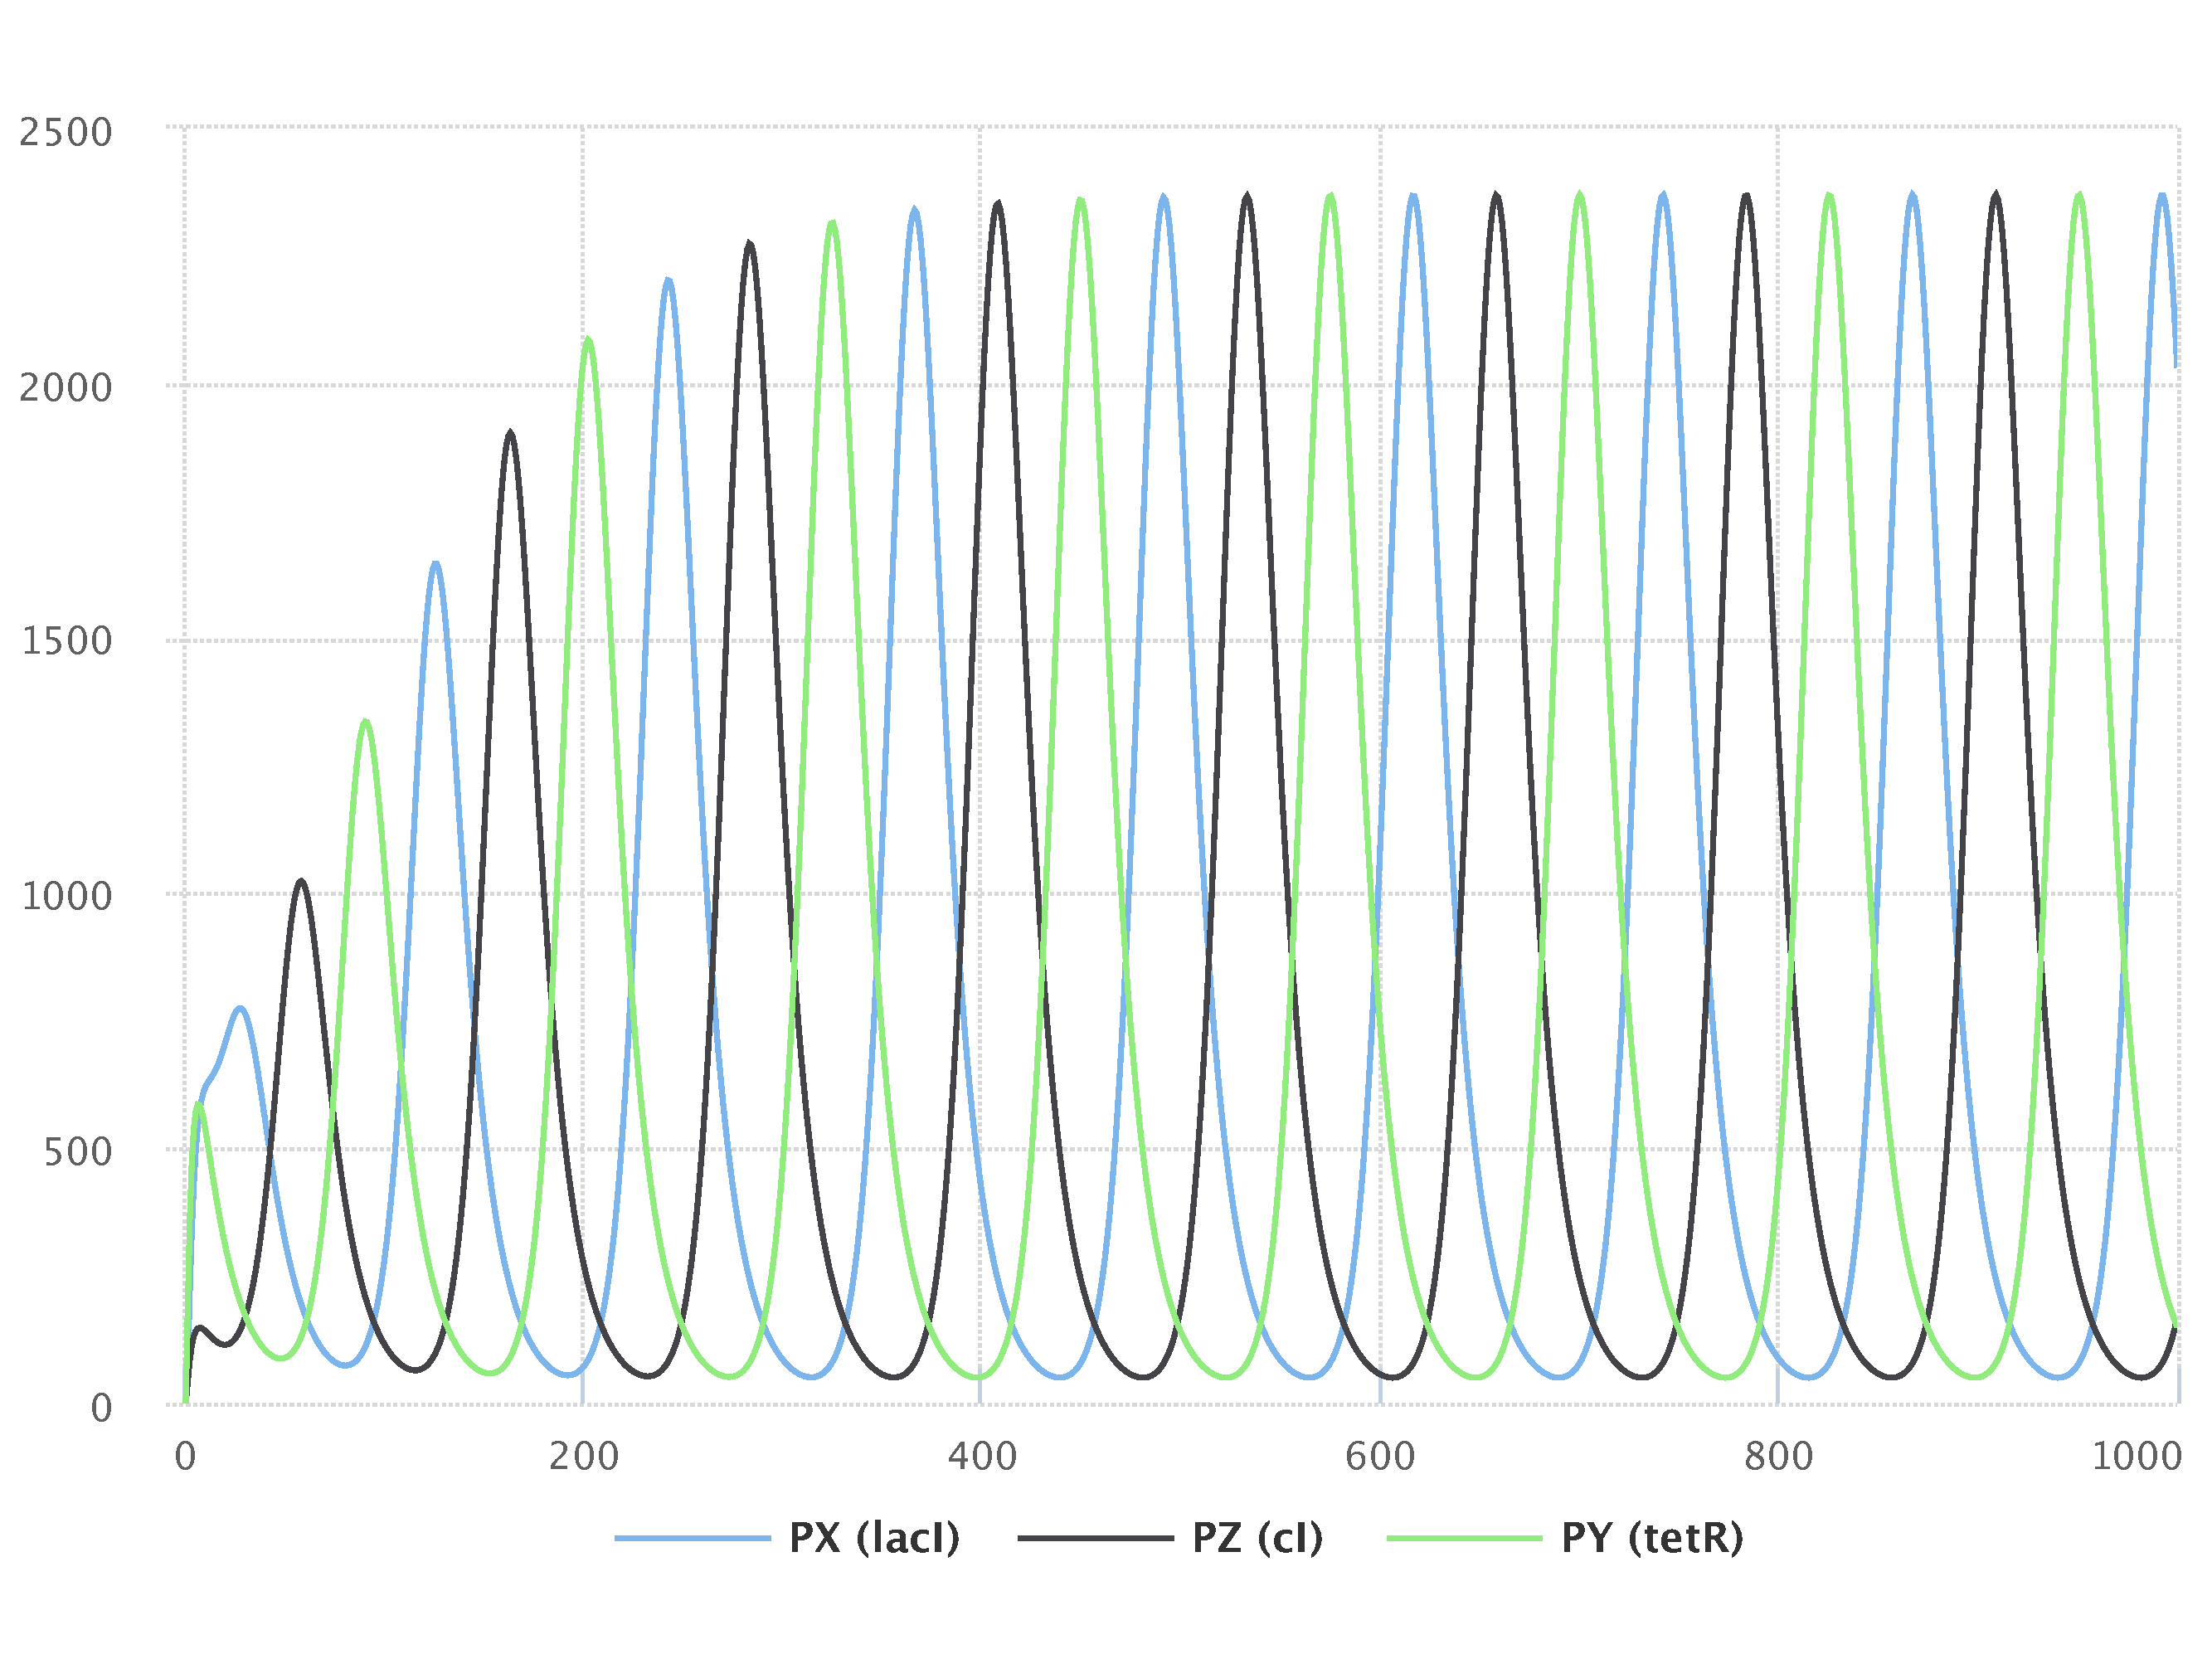
\includegraphics[width=1.0\textwidth]{examples/repressilator/results/sedml_webtools/timecourse}
        \caption{Time-course simulation of the repressilator depicting repressor proteins lacI, tetR and cI. Simulation with SED-ML web tools \citep{bergmann2017sed}.}
        \label{fig:rep_tc1}
    \end{minipage}\hfill
    \begin{minipage}{0.47\textwidth}
        \centering
        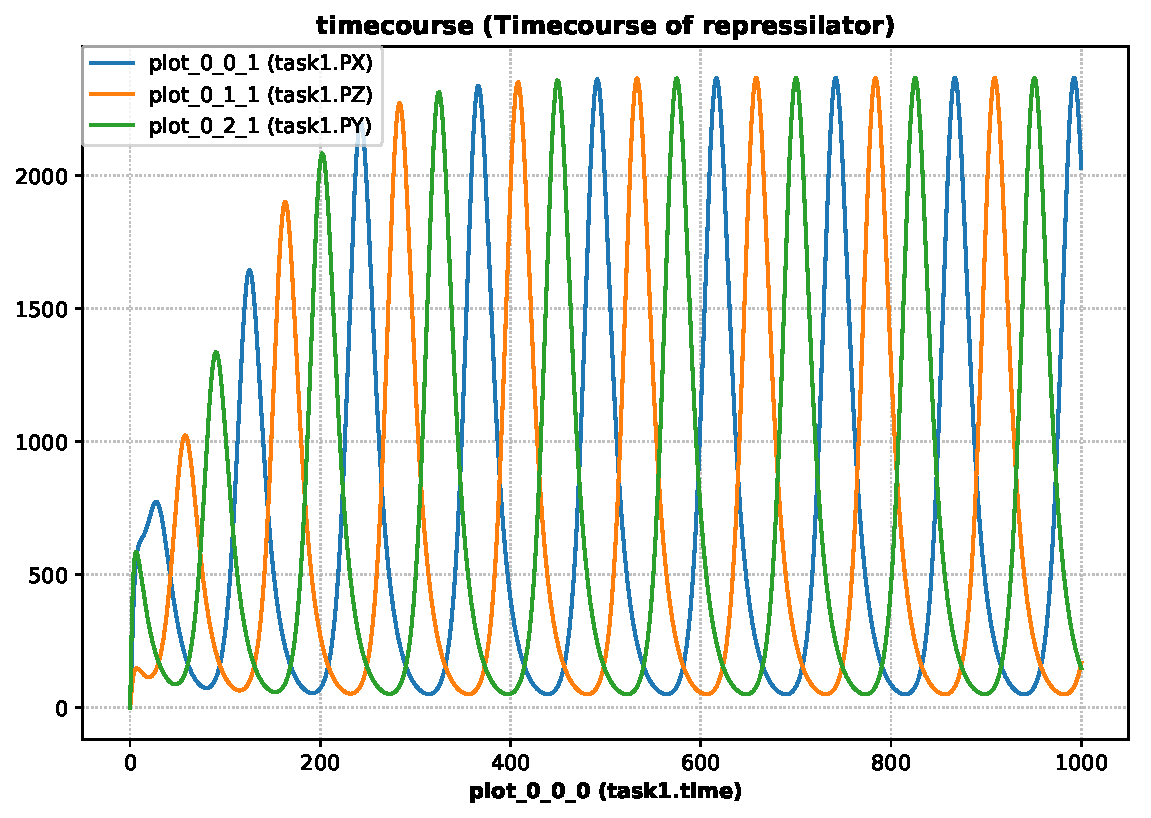
\includegraphics[width=1.0\textwidth]{examples/repressilator/results/tellurium/timecourse}
        \caption{Time-course simulation of the repressilator depicting repressor proteins lacI, tetR and cI. Simulation with tellurium \citep{tellurium}.}
        \label{fig:rep_tc2}
    \end{minipage}
\end{figure}


%% ~~ PRE-PROCESSING ~~
\subsection{Applying pre-processing}
\label{sec:preprocessing}
Often in simulation experiments model parameters are adjusted before simulation. When changing the parameter values for the protein copies per promoter \code{tps$\_$repr} and the leakiness in protein copies per promoter \code{tps$\_$active} like stated below, the system's behavior switches from sustained oscillations to damped oscillations towards an asymptotic steady-state. The model changes leading to that behavior are described as: 

\begin{enumerate}
	\item{Import the model as above.}
	\item{Change the value of the parameter \code{tps$\_$repr} from \code{0.0005} to \code{1.3e-05}.}
	\item{Change the value of the parameter \code{tps$\_$active} from \code{0.5} to \code{0.013}.}
	\item{Select a deterministic method.}
	\item{Run a uniform time course for the duration of 1000~min with an output interval of 1~min.}
	\item Plot the amount of lacI, tetR and cI against time in a 2D Plot.
\end{enumerate}

\fig{rep_pre1} and \fig{rep_pre2} show the results of the simulation.

\begin{figure}[ht]
    \centering
    \begin{minipage}{0.47\textwidth}
        \centering
        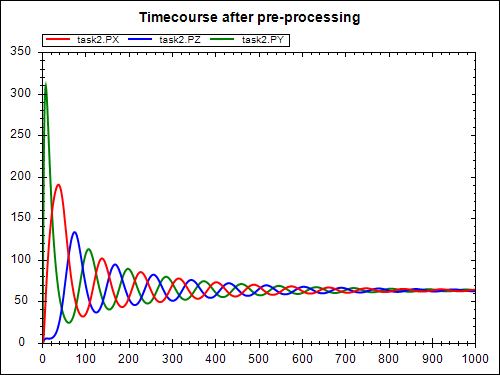
\includegraphics[width=1.0\textwidth]{examples/repressilator/results/sedml_webtools/preprocessing}
        \caption{Time-course simulation of the repressilator after changing parameters \code{tps$\_$repr} and \code{tps$\_$active}. Simulation with SED-ML web tools \citep{bergmann2017sed}.}
        \label{fig:rep_pre1}
    \end{minipage}\hfill
    \begin{minipage}{0.47\textwidth}
        \centering
        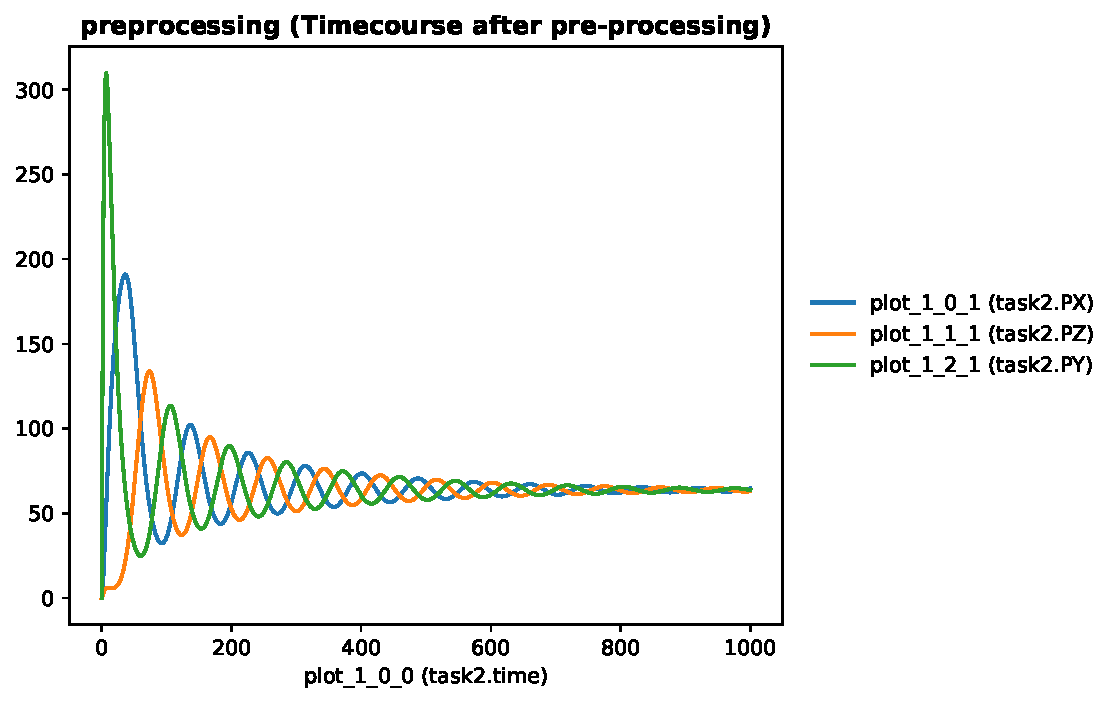
\includegraphics[width=1.0\textwidth]{examples/repressilator/results/tellurium/preprocessing}
        \caption{Time-course simulation of the repressilator after changing parameters \code{tps$\_$repr} and \code{tps$\_$active}. Simulation with tellurium \citep{tellurium}.}
        \label{fig:rep_pre2}
    \end{minipage}
\end{figure}


%% ~~ POST-PROCESSING ~~
\subsection{Applying post-processing}
\label{sec:postprocessing}
The raw numerical output of the simulation steps may be subjected to data post-processing before plotting or reporting. In order to describe the production of a normalized plot of the time-course in the first example (section \ref{sec:timecourse}), depicting the influence of one variable on another (in phase-planes), one performs the additional steps:

(Please note that the description steps 1 - 4 remain as given in section \ref{sec:timecourse} above.)
\begin{enumerate}
	\item[5.]{Collect \code{lacI(t)}, \code{tetR(t)} and \code{cI(t)}.}
	\item[6.]{Compute the highest value for each of the repressor proteins, \code{max(lacI(t))}, \code{max(tetR(t))}, \code{max(cI(t))}.}
	\item[7.]{Normalize the data for each of the repressor proteins by dividing each time point by the maximum value, i.e., \code{lacI(t)/max(lacI(t))}, \code{tetR(t)/max(tetR(t))}, and \code{cI(t)/max(cI(t))}.}
	\item[8.]{Plot the normalized \code{lacI} protein as a function of the normalized \code{cI}, the normalized \code{cI} as a function of the normalized \code{tetR} protein, and the normalized \code{tetR} protein against the normalized \code{lacI} protein in a 2D plot.}
\end{enumerate}

\fig{rep_post1} and \fig{rep_post2} show the result of the simulation after post-processing of the output data. 

\begin{figure}[ht]
    \centering
    \begin{minipage}{0.47\textwidth}
        \centering
        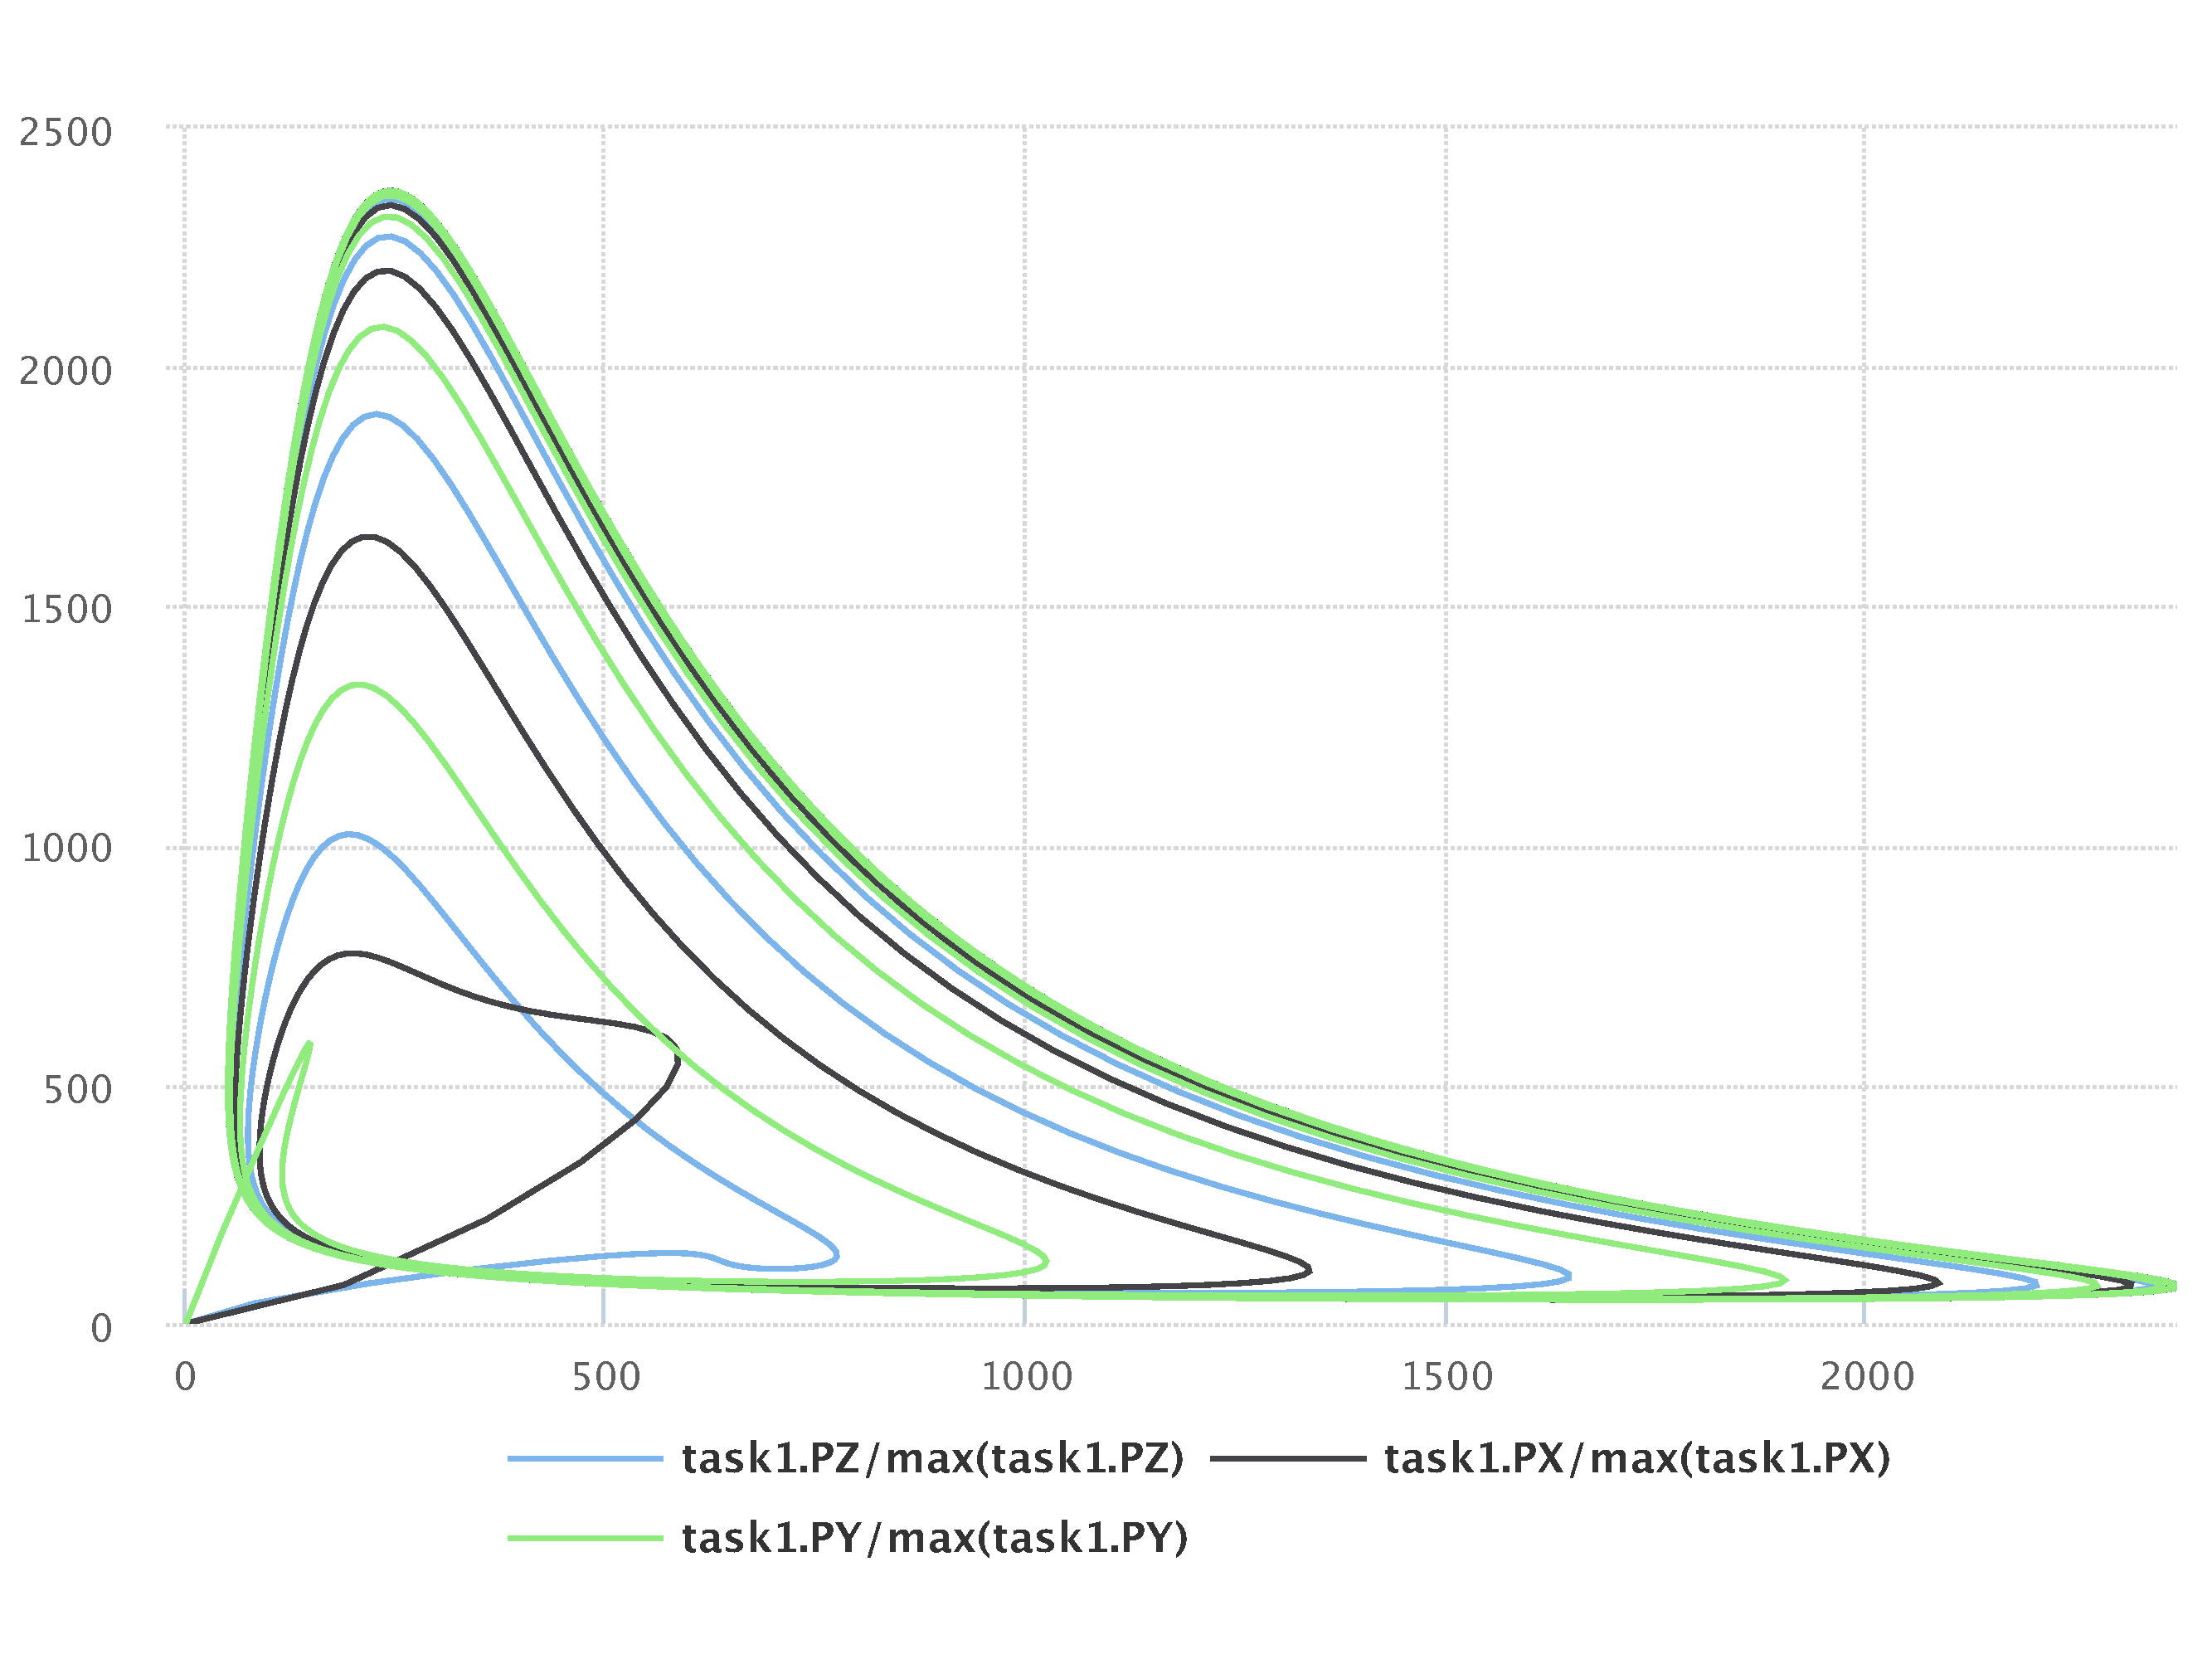
\includegraphics[width=1.0\textwidth]{examples/repressilator/results/sedml_webtools/postprocessing}
        \caption{Time-course simulation of the repressilator. Normalized \code{lacI}, \code{tetR} and \code{cI} in phase-plane. Simulation with SED-ML web tools \citep{bergmann2017sed}.}
        \label{fig:rep_post1}
    \end{minipage}\hfill
    \begin{minipage}{0.47\textwidth}
        \centering
        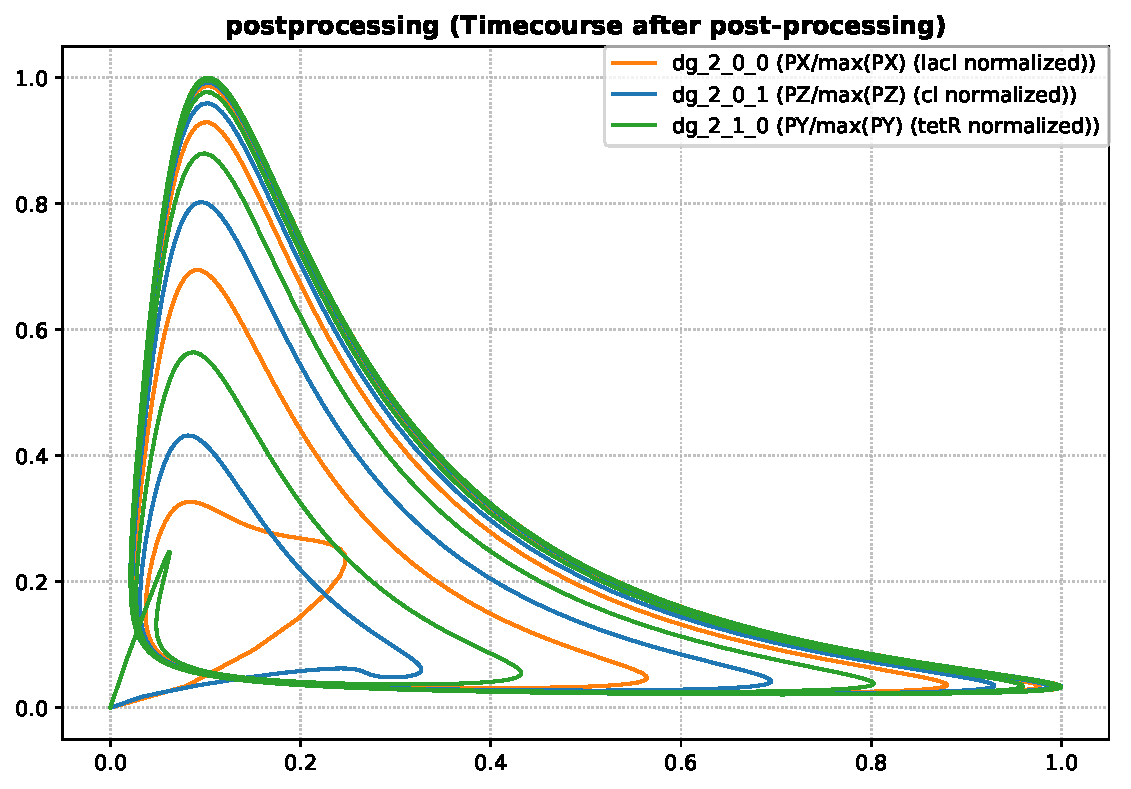
\includegraphics[width=1.0\textwidth]{examples/repressilator/results/tellurium/postprocessing}
        \caption{Time-course simulation of the repressilator. Normalized \code{lacI}, \code{tetR} and \code{cI} in phase-plane. Simulation with tellurium \citep{tellurium}.}
        \label{fig:rep_post2}
    \end{minipage}
\end{figure}
